\chapter{Java I/O}

 \begin{summary}
File handling is a fundamental aspect of programming, allowing developers to read from, write to, and manipulate files.  Java provides two primary APIs for file handling—the traditional java.io package and the more recent java.nio package. Understanding these APIs enables Java developers to efficiently manage data stored in files. 
 \end{summary}
 
 \section{Basics of File Handling}
 
A file system manages access to both the content of files and the metadata about those files.  Files are stored in directories.  The files and directories are accessed by specifying a path.  Paths are either absolute or relative:

\begin{itemize}
\item An absolute path is a path relative to the file system’s root directory. It’s expressed as the root directory symbol followed by a delimited hierarchy of directory names that ends in the target directory or file name.
\item A relative path is a path relative to some other directory. It’s expressed similarly to an absolute path but without the initial root directory symbol. In contrast, it’s often prefixed with one or more delimited “..” character sequences, where each sequence refers to a parent directory.
\end{itemize}

\begin{thm}[java.io.File]
        \url{https://docs.oracle.com/en/java/javase/21/docs/api/java.base/java/io/File.html}
    \end{thm}


\begin{lstlisting}
package be.pxl.ja;

public class Demo01 {

	public static final String SEPARATOR = System.getProperty("file.separator");

	public static void main(String[] args) {
		System.out.println("Current operating system: " + System.getProperty("os.name"));
		System.out.println("File separator: " + SEPARATOR);
		System.out.println("User's home directory: " + System.getProperty("user.home"));
		System.out.println("Current working directory: " + System.getProperty("user.dir"));
	}
}
\end{lstlisting}


On some systems,  Java can compensate for differences such as the direction of the file separator slashes in a pathname.  For example,  in the current implementation on Windows platforms,  Java accepts paths with either forward slashes or backslashes.
Thus, using forward slashes will make your application system independent.

\begin{lstlisting}
File file = new File("java/introduction.txt");
\end{lstlisting}


\begin{lstlisting}
import java.io.File;

public class PartitionSpace
{
   public static void main(String[] args)
   {
      File[] roots = File.listRoots();
      for (File root: roots)
      {
         System.out.println("Partition: " + root);
         System.out.println("Free space on this partition = " +
                            root.getFreeSpace());
         System.out.println("Usable space on this partition = " +
                            root.getUsableSpace());
         System.out.println("Total space on this partition = " +
                            root.getTotalSpace());
         System.out.println("***");
      }
   }
}
\end{lstlisting}


Like the legacy File class, Path also creates an object that may be used to locate a file in a file system.

\begin{thm}[java.nio.file.Path]
        \url{https://docs.oracle.com/en/java/javase/21/docs/api/java.base/java/nio/file/Path.html}
    \end{thm}
    
    
The utility class \textit{java.nio.files.Files} has a wide range of static method for file operations. 

\begin{thm}[java.nio.file.Files]
        \url{https://docs.oracle.com/en/java/javase/21/docs/api/java.base/java/nio/file/Files.html}
    \end{thm}


\begin{lstlisting}
// java.io API
boolean fileExists = file.exists();
boolean fileIsFile = file.isFile();
boolean fileIsDir = file.isDirectory();
boolean fileReadable = file.canRead();
boolean fileWritable = file.canWrite();
boolean fileExecutable = file.canExecute();
boolean fileHidden = file.isHidden();

// java.nio API
boolean pathExists = Files.exists(path);
boolean pathIsFile = Files.isRegularFile(path);
boolean pathIsDir = Files.isDirectory(path);
boolean pathReadable = Files.isReadable(path);
boolean pathWritable = Files.isWritable(path);
boolean pathExecutable = Files.isExecutable(path);
boolean pathHidden = Files.isHidden(path);
\end{lstlisting}

 
 \section{Accessing directories}
 
 The following program is used to display the names of all the files in a given folder.  It makes use of the File class.
 
 \begin{lstlisting}
 import java.io.File;

public class DisplayFiles {

    public static void main(String[] args) {
        // Check if a folder path has been provided as an argument
        if (args.length < 1) {
            System.out.println("Please provide a folder path as an argument.");
            return;
        }

        // Get the folder path from the command line arguments
        String folderPath = args[0];
        File folder = new File(folderPath);

        // Check if the folder exists and is indeed a directory
        if (!folder.exists() || !folder.isDirectory()) {
            System.out.println("The provided path does not exist or is not a directory.");
            return;
        }

        // List all files in the directory
        File[] listOfFiles = folder.listFiles();

        if (listOfFiles != null) {
            for (File file : listOfFiles) {
                if (file.isFile()) {
                    System.out.println(file.getName());
                }
            }
        } else {
            System.out.println("There was a problem reading the directory.");
        }
    }
}
\end{lstlisting}

A program with the same functionality can be written using the the java.nio classes. Pay special attention to the \textbf{try-with-resources statement.} The try-with-resources statement is a try statement that declares one or more resources. A resource is an object that must be closed after the program is finished with it. The try-with-resources statement ensures that each resource is closed at the end of the statement. Any object that implements java.lang.AutoCloseable, which includes all objects which implement java.io.Closeable, can be used as a resource.


\begin{figure}[H]
  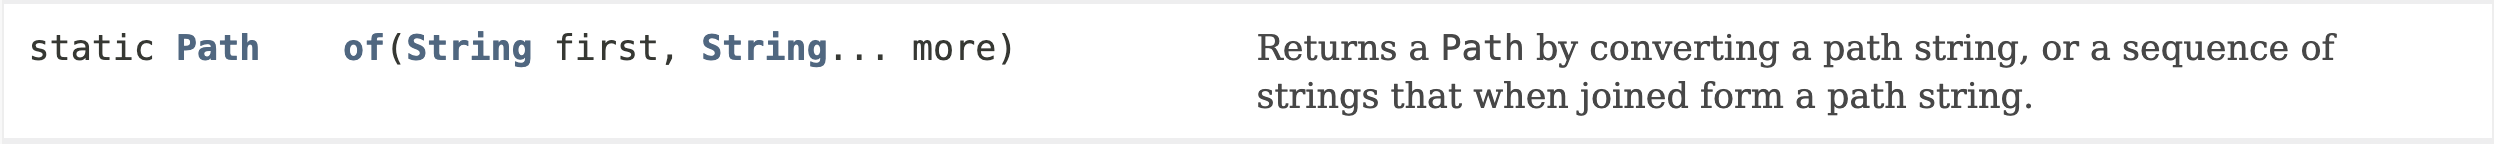
\includegraphics[width=\linewidth]{images/file_io/path_of.png}
  \caption{Static method in interface Path}
  \label{fig:paths}
\end{figure}

\begin{lstlisting}
import java.nio.file.Files;
import java.nio.file.Paths;
import java.nio.file.Path;
import java.io.IOException;
import java.util.stream.Stream;

public class DisplayFilesNIO {

    public static void main(String[] args) {
        // Check if a folder path has been provided as an argument
        if (args.length < 1) {
            System.out.println("Please provide a folder path as an argument.");
            return;
        }

        // Get the folder path from the command line arguments
        String folderPath = args[0];
        Path path = Paths.get(folderPath);

        // Check if the path exists and is a directory
        if (!Files.exists(path) || !Files.isDirectory(path)) {
            System.out.println("The provided path does not exist or is not a directory.");
            return;
        }

        // Use try-with-resources to ensure that the stream is closed
        try (Stream<Path> paths = Files.list(path)) {
            paths.forEach(filePath -> {
                if (Files.isRegularFile(filePath)) {
                    System.out.println(filePath.getFileName());
                }
            });
        } catch (IOException e) {
            System.out.println("An error occurred while reading the directory: " + e.getMessage());
        }
    }
}
\end{lstlisting}


\subsubsection{Creating directories and files}

The static method createDirectory() in the class Files can be used to create a new directory.

\begin{lstlisting}
import java.io.IOException;
import java.nio.file.Files;
import java.nio.file.Path;

public class Demo03CreatingDirectoriesAndFiles {

	public static void main(String[] args) {
		Path path = Path.of(System.getProperty("user.home"), "JavaAdvIO", "Opdracht3", "bijlage.txt");
		if (Files.notExists(path.getParent())) {
			try {
				Files.createDirectory(path.getParent());
			} catch (IOException e) {
				System.out.println("An error occured while creating directory " + path.getParent());
			}
		}
		if (Files.notExists(path)) {
			try {
				Files.createFile(path);
			} catch (IOException e) {
				System.out.println("An error occured while creating file " + path);
			}
		}
	}
}
\end{lstlisting}


\subsubsection{Reading small files}

For reading text files with a limited number of lines, you can use the static method readAllLines in the class Files.

\begin{lstlisting}
import java.nio.file.Path;
import java.nio.file.Paths;
import java.util.List;
import java.util.Random;

public class Demo04ReadingFiles {
	private static final Random RANDOM = new Random();

	public static void main(String[] args) {
		Path path = Paths.get("resources/small_file_with_text.txt");

		try {
			List<String> text = Files.readAllLines(path);
			System.out.println(text.get(RANDOM.nextInt(text.size())));
		} catch (IOException e) {
			e.printStackTrace();
		}
	}
}
\end{lstlisting}

\subsubsection{Copying files}

Creating a copy of a file is easy using the static method copy in the class Files.

\begin{lstlisting}
import java.io.IOException;
import java.nio.file.Files;
import java.nio.file.Path;
import java.nio.file.Paths;

public class Demo05CopyFiles {

	public static void main(String[] args) {
		Path original = Paths.get("resources/small_file_with_text.txt");
		Path copy = Paths.get("resources", "copy_" + System.currentTimeMillis() + ".txt");
		System.out.println(Files.exists(copy));
		try {
			Files.copy(original, copy);
			System.out.println(Files.exists(copy));
		} catch (IOException e) {
			e.printStackTrace();
		}
	}
}
\end{lstlisting}


\section{Byte Streams}

A stream is an ordered sequence of bytes of an arbitrary length.  Bytes flow over an output stream from an application to a destination and flow over an input stream from a source to an application.
The java.io package provides several output stream and input stream classes that are descendants of its abstract \textit{OutputStream} and \textit{InputStream} classes.


\begin{figure}[H]
  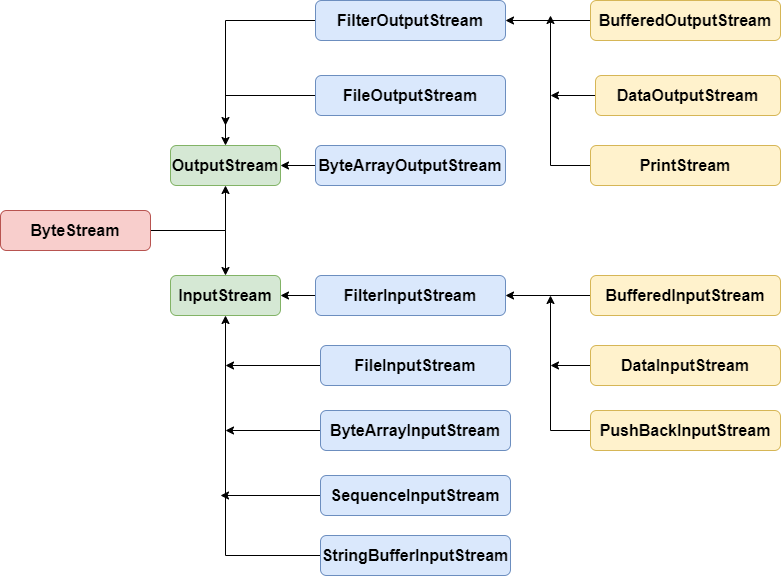
\includegraphics[width=\linewidth]{images/file_io/byte_stream_classes.png}
  \caption{Byte Streams}
  \label{fig:paths}
\end{figure}


\begin{lstlisting}
import java.io.FileOutputStream;
import java.io.IOException;

public class HexDataWriter {
    public static void main(String[] args) {
        // Example hexadecimal data: Image header, random bytes, etc.
        byte[] hexData = new byte[]{(byte)0xBA, (byte)0xAD, (byte)0xF0, (byte)0x0D, (byte)0xDE, (byte)0xAD, (byte)0xBE, (byte)0xEF};

        try (FileOutputStream outputStream = new FileOutputStream("binarydata.bin")) {
            outputStream.write(hexData);
            System.out.println("Hexadecimal data has been written to the file.");
        } catch (IOException e) {
            System.out.println("An error occurred.");
            e.printStackTrace();
        }
    }
}
\end{lstlisting}


\begin{lstlisting}
import java.io.FileInputStream;
import java.io.IOException;

public class HexDataReader {
    public static void main(String[] args) {
        try (FileInputStream inputStream = new FileInputStream("binarydata.bin")) {
            int byteRead;
            while ((byteRead = inputStream.read()) != -1) {
                // Convert the byte to a hexadecimal string
                System.out.print(String.format("%02X ", byteRead));
            }
        } catch (IOException e) {
            System.out.println("An error occurred.");
            e.printStackTrace();
        }
    }
}
\end{lstlisting}


\section{Character Streams}

A character set or charset is a set of characters and the encoding defines how these characters are stored in memory,  using one or more bytes.
If you need to stream characters, you should take advantage of Java’s writer and reader classes, which were designed to support character I/O (they work with char instead of byte). Furthermore, the writer and reader classes take character encodings into account.


\begin{figure}[H]
  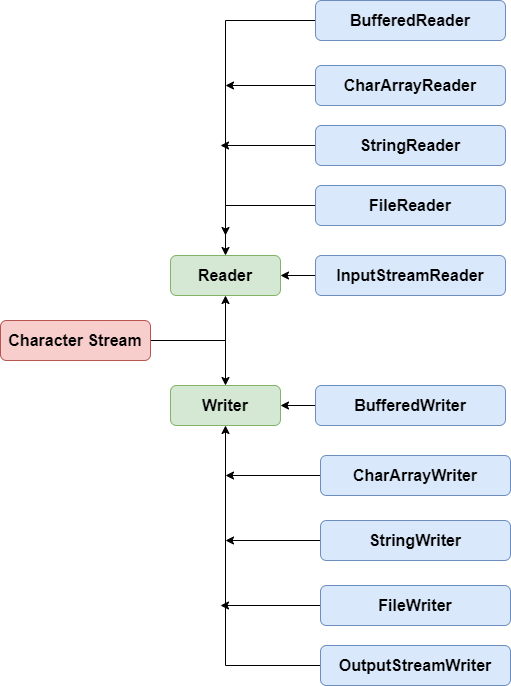
\includegraphics[width=\linewidth]{images/file_io/character_stream_classes.png}
  \caption{Byte Streams}
  \label{fig:paths}
\end{figure}


\subsection{BufferedReader}

The BufferedReader class offers a simple and efficient way to read larger text files. It groups (buffers) characters from a file so that you can read the file line by line. The newBufferedReader() method from the Files class simplifies the creation of the BufferedReader. The end of the text file is reached when readLine() returns null.

\begin{figure}[H]
  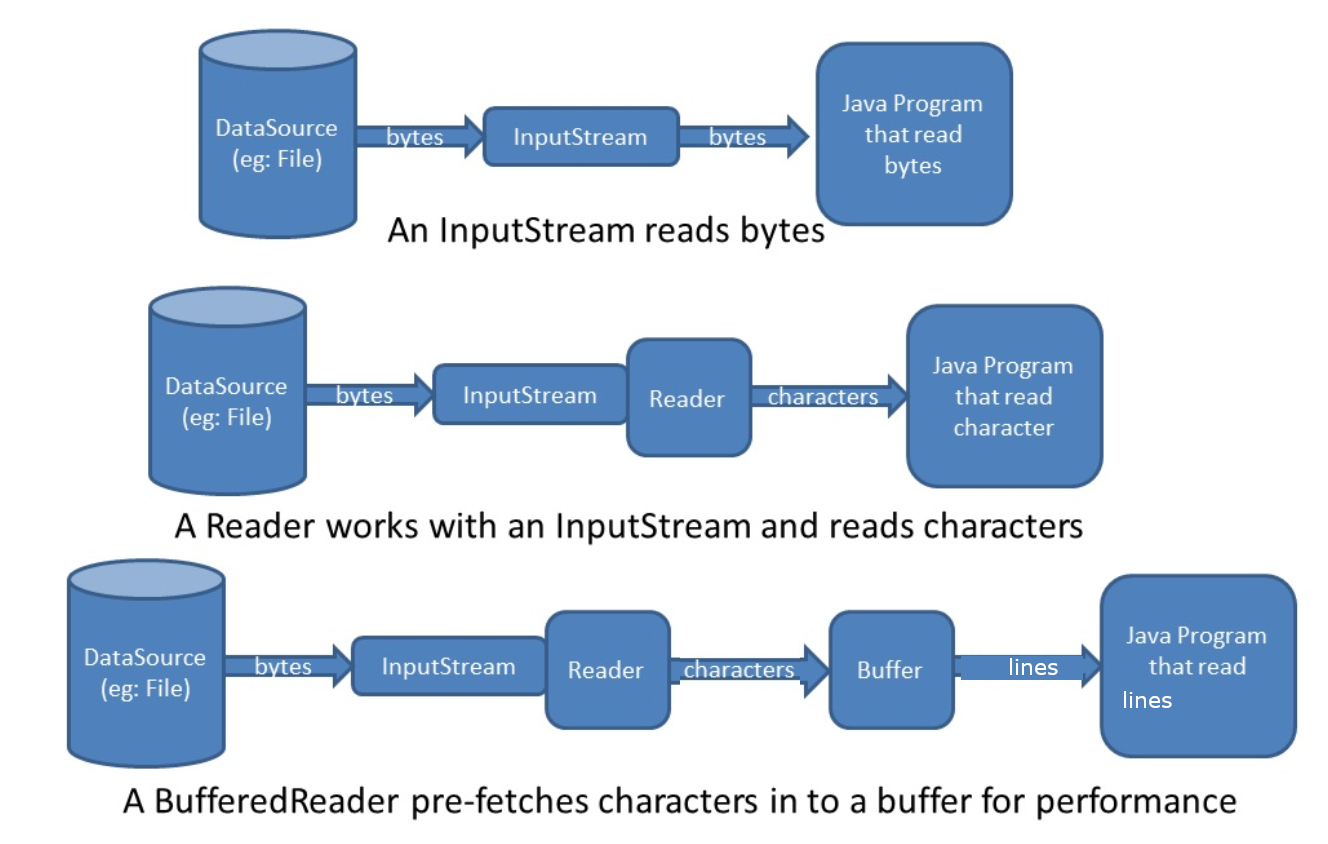
\includegraphics[width=\linewidth]{images/file_io/stream_reader.png}
  \caption{InputStream, InputStreamReader en BufferedReader}
  \label{fig:paths}
\end{figure}

\begin{lstlisting}
import java.io.BufferedReader;
import java.io.IOException;
import java.nio.file.Files;
import java.nio.file.Paths;

public class Demo06BufferedReader {

	public static void main(String[] args) {

		try (BufferedReader reader =  Files.newBufferedReader(Paths.get("resources/big_file_with_text.txt"))) {
			String line = null;
			while ((line = reader.readLine()) != null) {
				System.out.println(line);
			}
		} catch (IOException e) {
			e.printStackTrace();
		}
	}
}
\end{lstlisting}

\subsection{BufferedWriter}


Instead of writing to a file character by character, BufferedWriter writes larger pieces of text to the file at once.

\begin{lstlisting}
import java.nio.file.Files;
import java.nio.file.Paths;
import java.nio.file.StandardOpenOption;
import java.io.BufferedWriter;
import java.io.IOException;

public class NIOBufferedWriterExample {
    public static void main(String[] args) {
        // Path to the file
        String filePath = "example_nio.txt";

        // Using try-with-resources to ensure the BufferedWriter is closed after use
        try (BufferedWriter writer = Files.newBufferedWriter(Paths.get(filePath), 
                StandardOpenOption.CREATE, StandardOpenOption.WRITE)) {
            // Generating and writing 10 lines of text to the file
            for (int i = 1; i <= 10; i++) {
                String text = "Line " + i + ": This is an example of using Files.createBufferedWriter in Java.\n";
                writer.write(text);
            }
            System.out.println("Text has been written to " + filePath);
        } catch (IOException e) {
            System.out.println("An error occurred.");
            e.printStackTrace();
        }
    }
}
\end{lstlisting}

The options StandardOpenOption.CREATE and StandardOpenOption.WRITE specify that if the file does not exist, it should be created. If the file already exists, it will be opened for writing.

\subsection{Character sets}

\begin{lstlisting}
import java.nio.charset.Charset;

public class DefaultCharset {

	public static void main(String[] args) {

		System.out.println(Charset.defaultCharset().displayName());
	}

}
\end{lstlisting}

A charset specifies how characters are encoded into bytes and decoded back into characters.


\begin{lstlisting}
Files.newBufferedWriter(Paths.get("resources/myfile.txt"), Charset.forName("UTF-8"));
\end{lstlisting}

In UTF-8 1 to 4 bytes are used to represent the characters.


\begin{oefening}
A text message has been encoded by replacing each character of the message with an integer.  Each integer is an index into a key-phrase that contains all the lower case letters of the alphabet as well as the space character. The key-phrase may contain the same character in several locations. The encoded text is series of integers, like this:

\begin{verbatim}
35 10 10 33 9 24 3 17 41 8 3 20 51 16 38 44 47 32 33 10 19 38 35 28 49 
\end{verbatim}

To decode the message,  use each integer as an index in the key-phrase and output the corresponding character. For example, say that the key-phrase is this (the index of each character has been written above it):

\begin{verbatim}
          111111111122222222223333333333444444444455
0123456789012345678901234567890123456789012345678901 
six perfect quality black jewels amazed the governor
\end{verbatim}

using each integer from the encoded text as an index into the phrase
 results in the decoded message:

\begin{verbatim}
attack the bridge at dawn
\end{verbatim}

Write a program that decodes a secret message contained in a text file. The first line of the text file contains the key-phrase. Then the file contains a sequence of integers, each of which indexes the key-phrase. Find the character corresponding to each integer and output the secret message. Note if a character character such as `e' occurs several places in the key-phrase it may be encoded as different integers in different parts of the secret message.

(The recipient of the secret message gets only the file of integers and must put the key-phrase at the top of the file.) For example, here is the contents of a secret message file ready for the program:

\begin{verbatim}
six perfect quality black jewels amazed the governor
35 10 10 33 9 24 3 17 41 8 3 20 51 16 38 44 47 32 33 10 19 38 35 28 49 
\end{verbatim}

Here is a sample run of the program:

\begin{verbatim}
C:\> java Decode < secretFile.txt

attack the bridge at dawn
\end{verbatim}


Here is another secret message file, with key-phrase inserted, that you can use to test your program:

\begin{verbatim}
six perfect quality black jewels amazed the governor
31 16 2 3 4 42 48 7 27 9 10 43 12 13 35 15 1 40 18 3 
20 15 33 23 24 32 26 29 28 27 21 31 25 14 34 14 36 
42 38 19 40 41 27 3 44 50 46 42 48 49 50 6
\end{verbatim}

\end{oefening}


\section{Program properties}

It's a good idea to make Java programs easily configurable. To achieve this, parameters consisting of a key and a value are usually sufficient. In Java, you use the java.util.Properties class to read and write configuration files. You use the load method to read a configuration file and store to write the properties. With the getProperty method, you can request the corresponding value using a key.

\begin{lstlisting}
import java.io.IOException;
import java.io.InputStream;
import java.io.OutputStream;
import java.nio.file.Files;
import java.nio.file.Path;
import java.util.Properties;
import java.util.Scanner;

public class Demo08ProgramWithProperties {
	private static final String CONFIG_FILE = "resources/config.properties";

	public static void main(String[] args) {
		try(InputStream inputStream = Files.newInputStream(Path.of(CONFIG_FILE))) {
			Properties properties = new Properties();
			properties.load(inputStream);
			System.out.println("Welcome " + properties.getProperty("demo.name") + "!");
			System.out.println("You're mails will be sent to: " + properties.getProperty("demo.email"));
		} catch (IOException e) {
			createProperties();
		}
	}

	private static void createProperties() {
		Scanner scanner = new Scanner(System.in);
		System.out.println("You're using this program for the first time.");
		System.out.println("What's your name:");
		String name = scanner.nextLine();
		System.out.println("What's your company:");
		String company = scanner.nextLine();
		System.out.println("What's your email:");
		String email = scanner.nextLine();
		Properties properties = new Properties();
		properties.setProperty("demo.name", name);
		properties.setProperty("demo.company", company);
		properties.setProperty("demo.email", email);
		try(OutputStream outputStream = Files.newOutputStream(Path.of(CONFIG_FILE))) {
			properties.store(outputStream, "Demo program configuration");
		}
		catch (IOException e) {
			System.out.println("We were not able to save your configuration.");
		}
	}
}
\end{lstlisting}

The first time the program is executed, the config.properties file is not yet present. The user is then asked to enter the information.

\begin{verbatim}
You're using this program for the first time.
What's your name:
Nele
What's your company:
PXL
What's your email:
nele.custers@pxl.be
\end{verbatim}

You will see that after running the program, a file \textit{resources/config.properties} has been created. This file contains the following information.

\begin{verbatim}
#Demo program configuration
#Tue Nov 17 09:13:51 CET 2020
demo.name=Nele
demo.company=PXL
demo.email=nele.custers@pxl.be
\end{verbatim}

When you restart the program, the .properties file is read, and you'll get the following output.

\begin{verbatim}
Welcome Nele!
You're mails will be sent to: nele.custers@pxl.be
\end{verbatim}


\section{Object serialization and deserialization}

Object serialization in Java is the process of converting an object's state into a byte stream, thus enabling the object to be easily saved to a file or transmitted over a network. Deserialization, on the other hand, is the reverse process, where the byte stream is converted back into a replica of the original object, restoring its state. This mechanism allows for the persistent storage of objects and the exchange of objects between Java systems.

\subsection{Object serialization}
To serialize an object in Java, the class must implement the java.io.Serializable interface, which is a marker interface (it does not contain any method declarations) indicating that an object of this class can be serialized. Here is a simple example:

\begin{lstlisting}
import java.io.*;

public class User implements Serializable {
    private String name;
    private transient int age; // the transient keyword indicates that this field should not be serialized

    public User(String name, int age) {
        this.name = name;
        this.age = age;
    }
    
    // Getters and Setters
}

// Serialization process
try (ObjectOutputStream oos = new ObjectOutputStream(new FileOutputStream("user.ser"))) {
    User user = new User("John Doe", 30);
    oos.writeObject(user);
} catch (IOException e) {
    e.printStackTrace();
}
\end{lstlisting}

\subsection{Object deserialization}


Deserialization converts the byte stream back into an object, as shown in the following example:

\begin{lstlisting}
import java.io.*;

public class DeserializeExample {
    public static void main(String[] args) {
        try (ObjectInputStream ois = new ObjectInputStream(new FileInputStream("user.ser"))) {
            User user = (User) ois.readObject();
            System.out.println("Name: " + user.getName() + ", Age: " + user.getAge());
        } catch (IOException | ClassNotFoundException e) {
            e.printStackTrace();
        }
    }
}
\end{lstlisting}

In this example, the User class must implement the Serializable interface. Note the use of transient with the age variable; it indicates that this field should not be serialized. During deserialization, the age field of the deserialized User object will not be restored to its original value but will be set to the default value for its type (0 in this case).


%\subsection{Audio en afbeeldingen}

% expand on performance, security, concurrency

%exercises:
% file search Files.walk
% log file analyzer with very large log files
% GZIPOutputStreams for file compression


\section{Best practices}

Here are some best practices for reading and writing to files using Java libraries:

\begin{itemize}

\item \textbf{Use try-with-resources}: When reading or writing to a file, it's important to properly handle the opening and closing of the file stream.  Java 7 introduced the try-with-resources statement which automatically closes the file stream once the code block is executed.

\item \textbf{Use buffered streams}: Reading or writing large files can be a performance bottleneck. Using buffered streams can help improve performance by reducing the number of I/O operations required.

\item \textbf{Handle exceptions}: When reading or writing to a file, it's important to handle any exceptions that may occur. Common exceptions include FileNotFoundException and IOException.

\item \textbf{Use appropriate encoding}: When reading or writing text files, it's important to use the appropriate encoding. The default encoding used by Java is usually UTF-8, but this may not be appropriate for all scenarios.

\item \textbf{Use relative paths}: When working with files, it's best to use relative paths instead of absolute paths. This makes the code more portable and easier to maintain.

\item \textbf{Check for file existence}: Before reading or writing to a file,  it's important to check if the file exists. This can be done using the File.exists() method.

\item \textbf{Use descriptive file names}: When creating new files, it's important to use descriptive file names that are easy to understand and maintain. This can help prevent naming conflicts and make it easier to find and manage files.
\end{itemize}


\begin{oefening}

\textbf{Exploring and Analyzing a Spring Boot Maven Project with Files.walk()}

Write a Java program that traverses a Spring Boot project directory using Files.walk(). Accept the project path from the user and validate that the directory exists.

\begin{verbatim}
java Explore C:\my-projects\secret-project
\end{verbatim}

Extract project structure components:
\begin{itemize}
\item Locate \textbf{pom.xml} and count the dependencies.
\item Identify application.properties.
\item Find Java source files (*.java) and count their occurrences.
\item Count the number of REST controller (@RestController)
\item Detect hardcoded credentials in application.properties. Use regex to check for password=, secret=, or key=.
\end{itemize}

Example output:
\begin{verbatim}
Project Structure:
- Found pom.xml at: secret-project/pom.xml
- Found 5 dependencies
- Found 25 Java files.
- Found 5 controller classes.

Security Checks:
- Hardcoded password detected in application.properties: "password=admin123"
\end{verbatim}

\end{oefening}

